\section{Memory pipeline}

\begin{figure}[H]
    \centering
    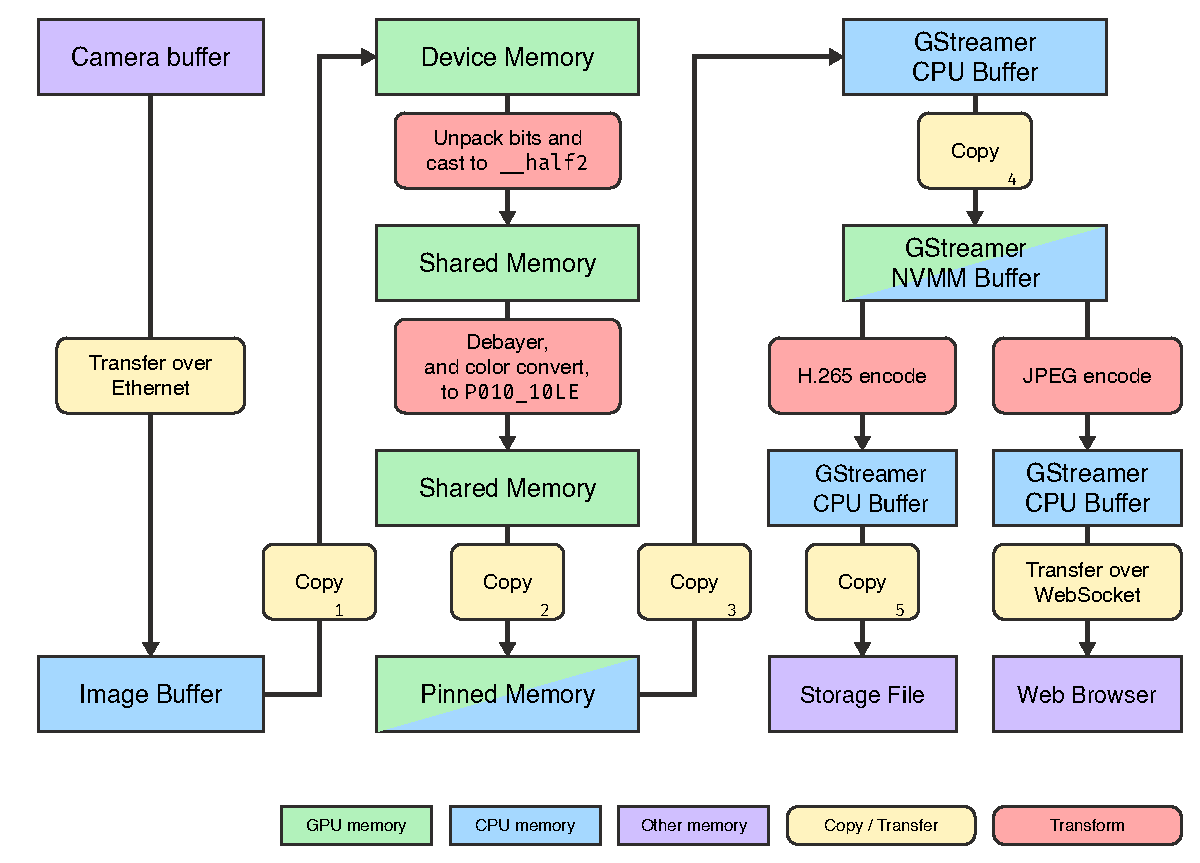
\includegraphics[width=\textwidth]{figures/memory_pipeline/current.pdf}
    \caption{Overview of the memory movement in the current pipeline.}
    \label{fig:pipeline_current}
\end{figure}



\subsection{Camera to Xavier}
The first step in the memory pipeline is to move the image buffers from the camera to the \jx.
As this link is the current bottleneck of the whole pipeline, it is important to optimize the performance as much as possible.

Firtsly, to get the best possible network performance on the \jx, several network configurations were performed as discussed Section\ref{sec:network_configuration}.

Secondly, the \cams have a multitude of differend settings that can be configured to optimize the performance.
One important step is to

The \cams have an internal Image buffer of 128MB, which is used to store the image data before it is sent to the \jx.
With 10-bit resolution per image the


\begin{align}
    \frac{128*1000000*8}{2048*2448*10}
\end{align}

\subsection{Image buffer to Device Memory}
Pinned host to host,
Pinned host to device,
Device host to device, -> nsys

\subsubsection{Device to Shared}
This is discussed thuroughly in Section




